
\begin{problem}
	You are given two bipartite graphs $G$ and $H$ below. For each
	graph determine whether it has a perfect matching.
	Justify your answer, either by 
	listing the edges that are in the matching or using
	Hall's Theorem to show that the graph does not have a
	perfect matching.

	\begin{center}
	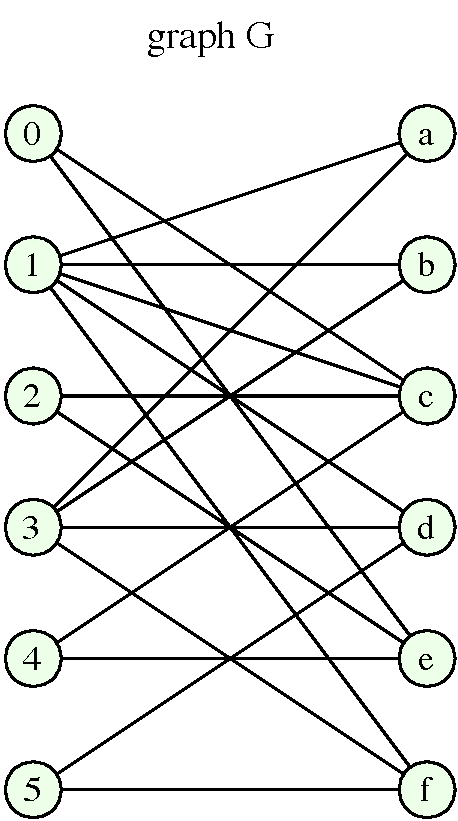
\includegraphics[width = 1.75in]{bipartite_graphG_hw5.pdf}
	\ \ \ \ \
	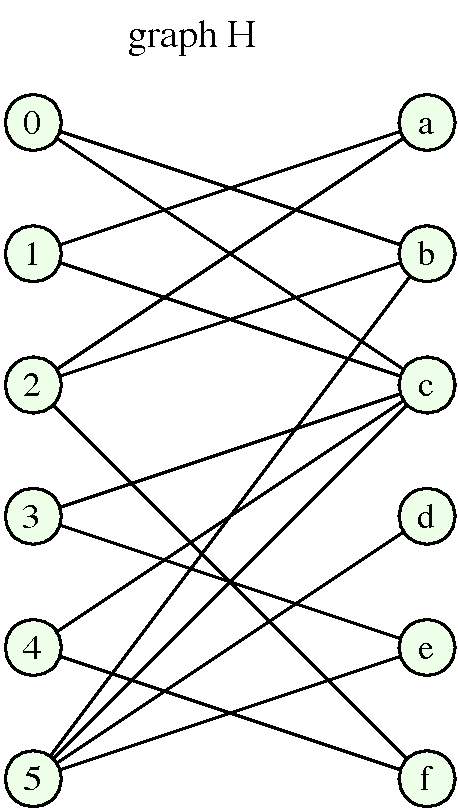
\includegraphics[width = 1.75in]{bipartite_graphH_hw5.pdf}
	\end{center}
\end{problem}

%%%%%%%%%%%%%%%%%%%%%%%%%%%%

% new


